\documentclass[17pt,mathserif]{beamer}
\usepackage{pdfrender}
\usepackage{tikz}
\usepackage{times}
\usepackage{caption}
\usepackage{textcomp}
%\usepackage{subcaption}
\usepackage{ifthen}
%\usepackage[backend=bibtex]{biblatex}
%\usepackage[style=authortitle,backend=bibtex]{biblatex}
\usepackage[style=authortitle-icomp,backend=bibtex]{biblatex}

\usetikzlibrary{shapes,arrows,mindmap,backgrounds}
%\usepackage{default}

%\geometry{paper=legalpaper}

\captionsetup[figure]{labelformat = empty, textfont={it}}

\graphicspath{{./Pictures/}}

\bibliography{bibliography}

\title{Computer Vision on the \\SpiNNaker Platform}
\author{Garibaldi Pineda Garc\'ia\\{\small Supervisor: Prof. Steve Furber}}
%\titlegraphic{
\includegraphics[scale=0.6]{./Pictures/manchester-logo}}
%\institute{The University of Manchester}
\institute{
\includegraphics[scale=0.6]{manchester-logo}
    \\The University of Manchester}

\date{}

% % % % % % % % % % % % % % % % % % % % % % % % % % % % % % % % % %

\usetheme{Pittsburgh}
\usecolortheme{seahorse}
%\definecolor{theme-color}{RGB}{33,84,157} %soothing blue
\definecolor{themecolor}{RGB}{64, 26, 86} %dark-manchester
\definecolor{manchester}{RGB}{80, 0, 127} %dark-manchester
\definecolor{darkgray}{gray}{0.15}

\setbeamercolor*{structure}{bg=themecolor!30,fg=themecolor}

\setbeamercolor*{palette primary}{use=structure,fg=white,bg=structure.fg}
\setbeamercolor*{palette secondary}{use=structure,fg=white,bg=structure.fg!80}
\setbeamercolor*{palette tertiary}{use=structure,fg=white,bg=black}
\setbeamercolor*{palette quaternary}{fg=white,bg=black}

\setbeamercolor{section in toc}{fg=black,bg=white}
\setbeamercolor{alerted text}{use=structure,fg=structure.fg!50!black!80!black}

\setbeamercolor{titlelike}{parent=palette primary,fg=structure.fg!50!black}
%\setbeamercolor{frametitle}{bg=themecolor!90,fg=white}
\setbeamercolor{frametitle}{bg=manchester}

\setbeamercolor*{titlelike}{parent=palette primary}

% % % % % % % % % % % % % % % % % % % % % % % % % % % % % % % % % %

\setbeamerfont{author}{size=\large}
\setbeamerfont{institute}{size=\footnotesize\itshape}
\setbeamerfont{title}{size=\fontsize{28}{38}}
\setbeamerfont{subtitle}{size=\Large\normalfont\slshape}
\setbeamerfont{caption}{size=\footnotesize}
\setbeamerfont{frametitle}{size=\fontsize{22}{26}}
%\setbeamerfont{itemize item}{size=\fontsize{30}{36}}

% % % % % % % % % % % % % % % % % % % % % % % % % % % % % % % % % %

\setbeamertemplate{title page}{%
    %    \setbeamerfont{author}{size=\Huge}
    %    \setbeamerfont{institute}{size=\normalsize\itshape}

    %    \setbeamerfont{subtitle}{size=\Large\normalfont\slshape}
    \begin{tikzpicture}[remember picture,overlay]
    \fill[themecolor]
    ([yshift=15pt]current page.west) rectangle (current page.south east);

    \node[anchor=east] 
    at ([yshift=-40pt]current page.north east) (author)
    {\parbox[t]{.8\paperwidth}{\raggedleft%
            \usebeamerfont{author}\textcolor{darkgray}{%
                \textpdfrender{
                    TextRenderingMode=FillStroke,
                    FillColor=darkgray,
                    LineWidth=.05ex,
                }{\insertauthor}}}};

    \node[anchor=north east] 
    at ([yshift=-60pt]current page.north east) (institute)
    {\parbox[t]{.78\paperwidth}{\raggedleft%
            \usebeamerfont{institute}\textcolor{gray}{\insertinstitute}}};

    \node[anchor=south west] 
    at ([yshift=20pt]current page.west) (logo)
    {\parbox[t]{.19\paperwidth}{\raggedleft%
            \usebeamercolor[fg]{titlegraphic}\inserttitlegraphic}};

    \node[anchor=west]
    at ([yshift=-40pt, xshift=0.1\paperwidth]current page.west) (title)
    {\parbox[t]{\textwidth}{\raggedleft%
            \usebeamerfont{title}\textcolor{white}{%
                \textpdfrender{
                    TextRenderingMode=FillStroke,
                    FillColor=white,
                    LineWidth=.08ex,
                }{\inserttitle}}}};

    \node[anchor=east]
    at ([yshift=-60pt,xshift=-20pt]current page.east) (subtitle)
    {\parbox[t]{.6\paperwidth}{\raggedleft\usebeamerfont{subtitle}\textcolor{black}{\insertsubtitle}}};
    \end{tikzpicture}
}
% % % % % % % % % % % % % % % % % % % % % % % % % % % % % % % % % %
\setbeamertemplate{frametitle}
{\vskip-3pt
    {
    \leavevmode
    \hbox{%
        \begin{beamercolorbox}[wd=\paperwidth,ht=1cm,dp=0.1cm]{frametitle}%
            
        \end{beamercolorbox}
        \hspace*{-\paperwidth}
        \begin{beamercolorbox}[wd=0.3\paperwidth,ht=1cm,dp=0.1cm]{frametitle}%
            \vspace*{-0.05cm}
            \hspace*{0.2cm}
            
\includegraphics[scale=0.5]{manchester-logo}
        \end{beamercolorbox}
     
        \begin{beamercolorbox}[wd=0.7\paperwidth,ht=1cm,dp=0.1cm, right]{frametitle}%
            \vspace*{0cm}
            \raggedright\hfill \insertframetitle %\normalsize\insertframetitle
            \hspace*{0.1cm}
        \end{beamercolorbox}
    }%
    }
    \hbox{%
        \begin{beamercolorbox}[wd=\paperwidth,ht=1cm,dp=0.1cm right]{yellow}%
            \vspace*{0.5cm}
            \raggedright\hfill \color<1>{darkgray}{\small\insertframesubtitle} \hspace*{1.6cm}
        \end{beamercolorbox}
    }%
}

% % % % % % % % % % % % % % % % % % % % % % % % % % % % % % % % % %

\usebackgroundtemplate%
{%
%\parbox{\linewidth}{
\tikz[overlay,remember picture] 
\node[at=(current page.south west),anchor=south west,inner sep=0.3cm] {
    
\includegraphics[scale=0.25]{spinnaker-logo}
};
%    \hfill
%    }
}

%\setbeamertemplate{footline}{%
%    \parbox{\linewidth}{
%        \vspace*{-60pt}
%        \hspace*{5pt}
%        
\includegraphics[scale=0.25]{spinnaker-logo}
%        \hfill}
%}


% % % % % % % % % % % % % % % % % % % % % % % % % % % % % % % % % %

\setbeamertemplate{itemize items}{$\circ$}
\setbeamertemplate{itemize subitem}[circle]
\setbeamertemplate{itemize subsubitem}[triangle]

% % % % % % % % % % % % % % % % % % % % % % % % % % % % % % % % % %

\begin{document}
    {
        \setbeamertemplate{footline}{} 
        \begin{frame}
            \titlepage
        \end{frame}
    }
    
%    \begin{frame}{Broad PhD goals}
%        %More content goes here
%        \vspace*{-3em}
%        \begin{itemize}
%            \item Computer vision on neural networks
%            \item 
%            \item 
%        \end{itemize}
%    \end{frame}
    

    \begin{frame}{Why vision?} %{hello}
      %More content goes here
        \vspace*{-3em}
        \begin{center}
            \textit{{ A picture is worth a thousand words}}
            \vspace*{-0.8em}
            \begin{figure}
                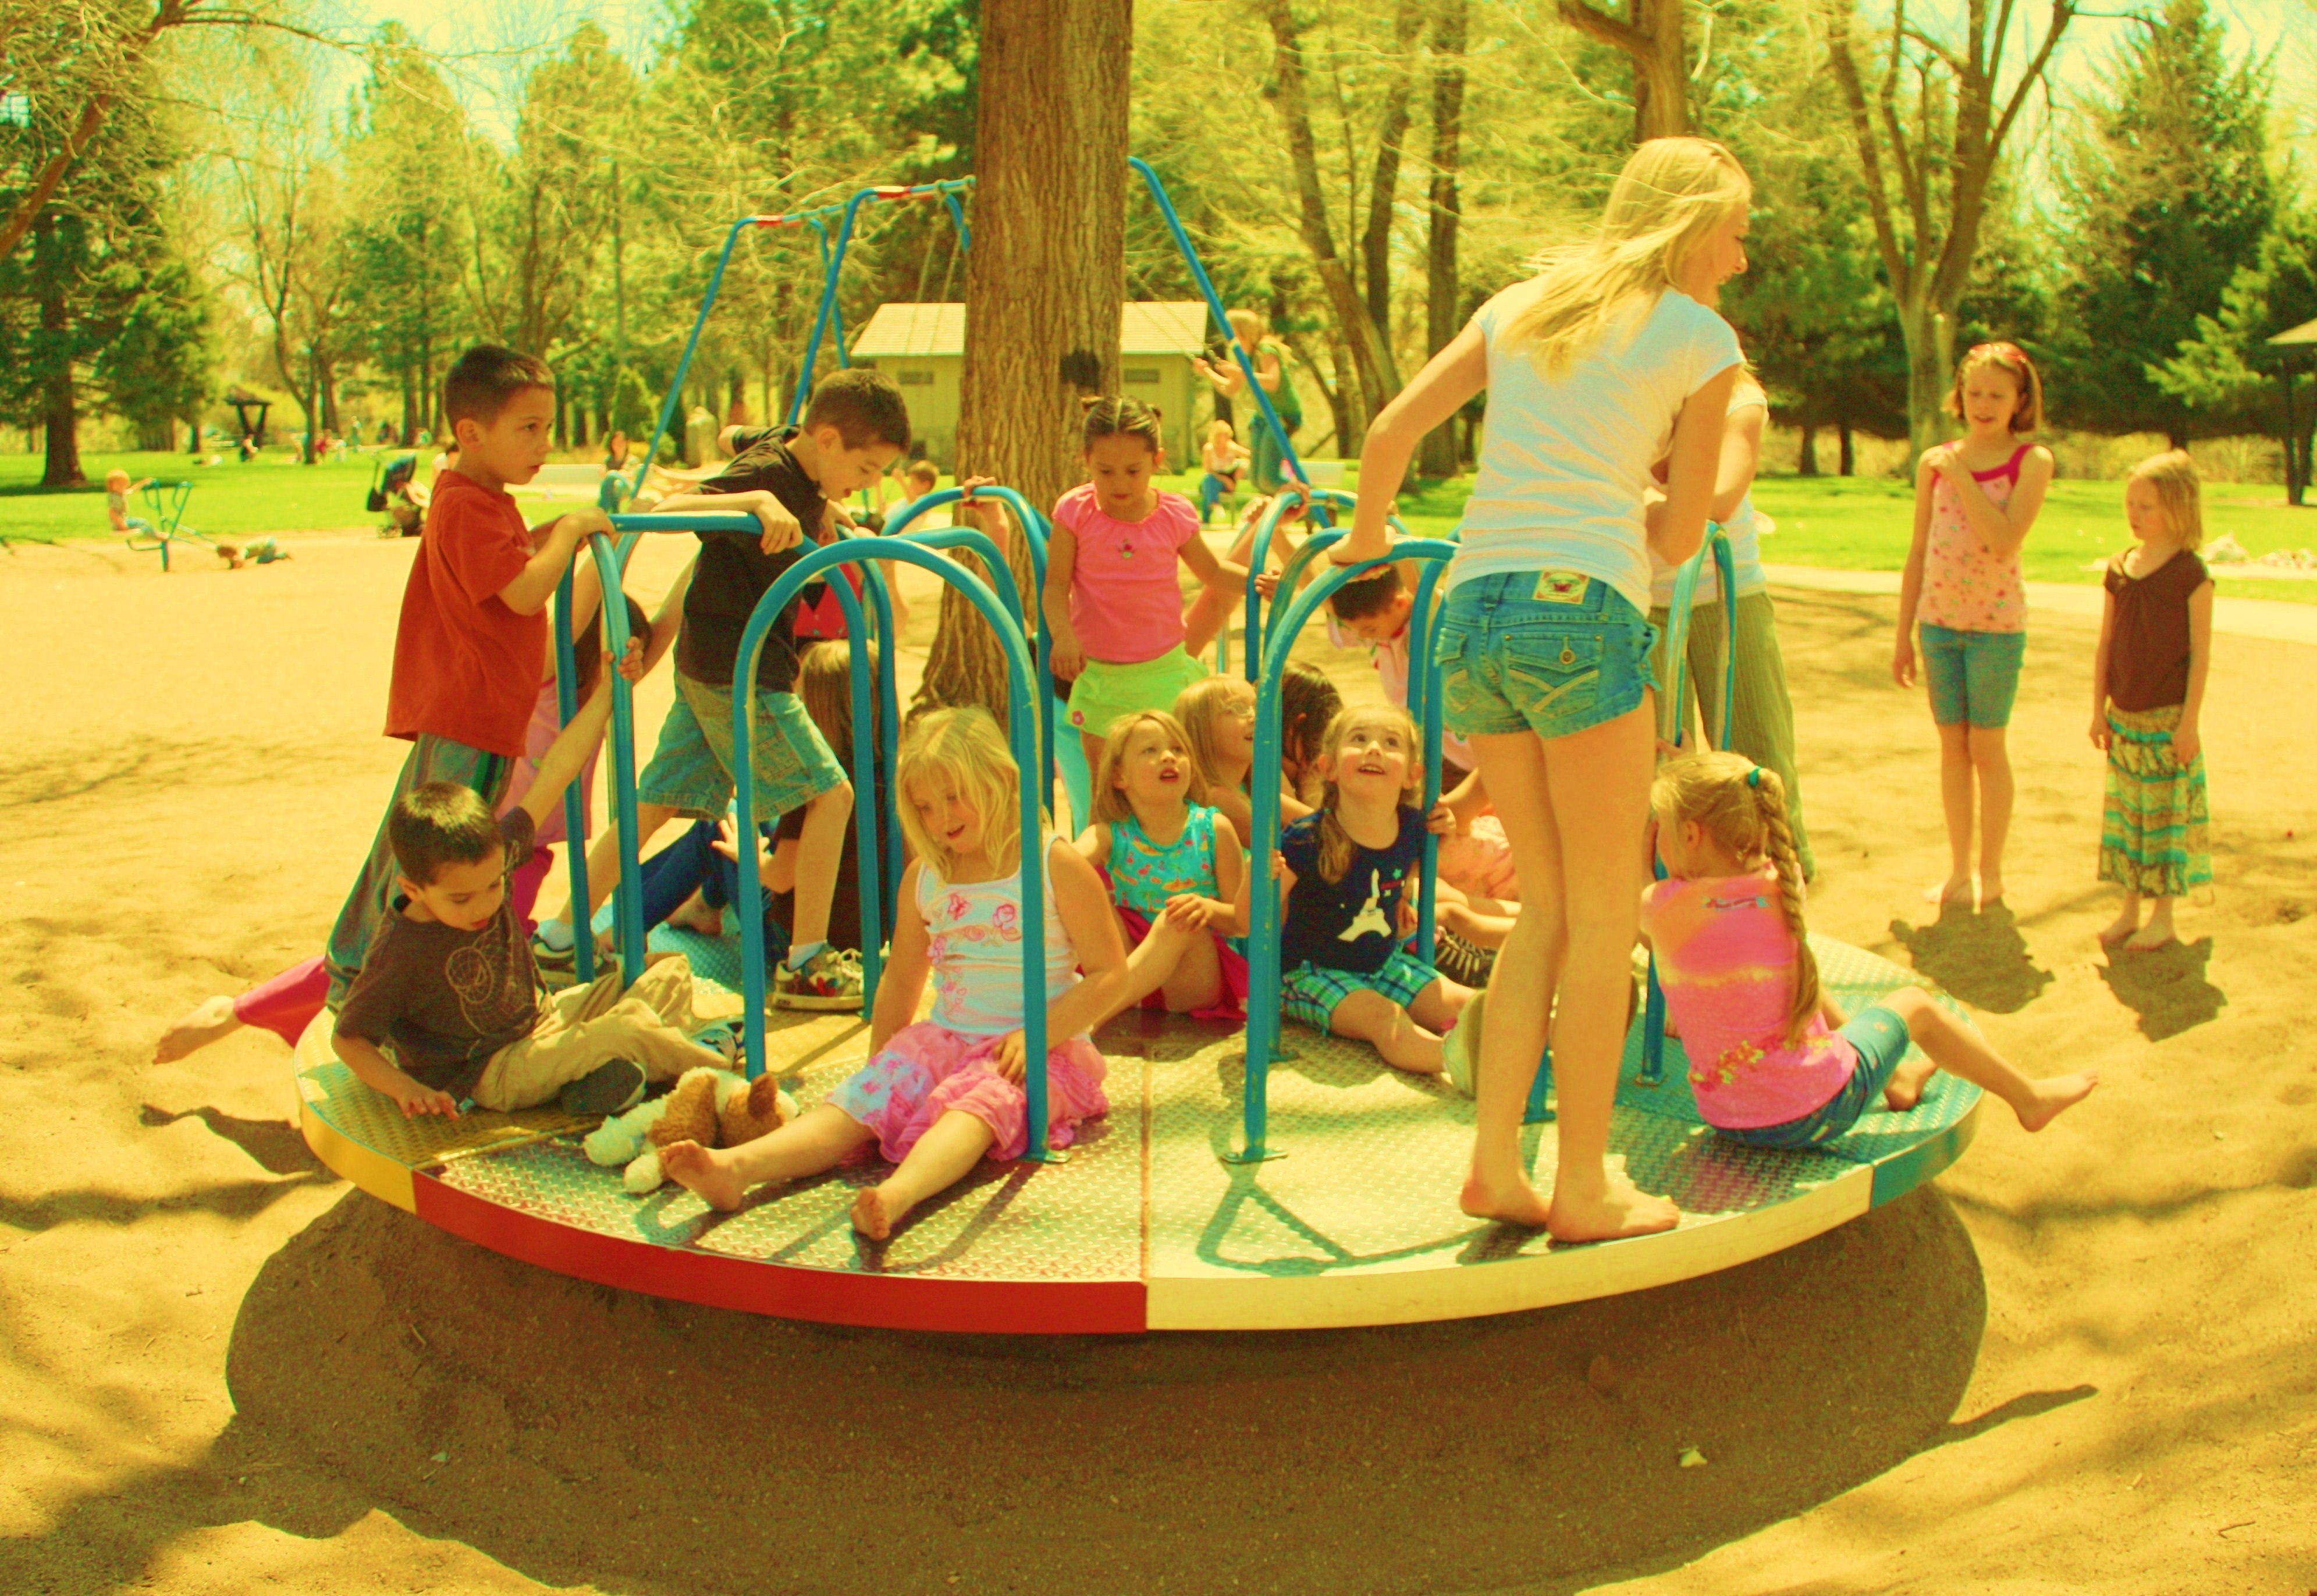
\includegraphics[scale=0.06]{./children_playing}
            \end{figure}
        \end{center}

    \end{frame}
    

    \begin{frame}{Why SpiNNaker?} %{hello}
        %More content goes here
        \vspace*{-3em}        
        \begin{columns}[c] % the "c" option specifies center vertical alignment
            \column{.666\textwidth} % column designated by a command
            \begin{itemize}
                \item Spiking Neural Network Architecture 
                \item Massively parallel processing
                \item Network capabilities
            \end{itemize}
            \column{.333\textwidth}
            \begin{figure}
                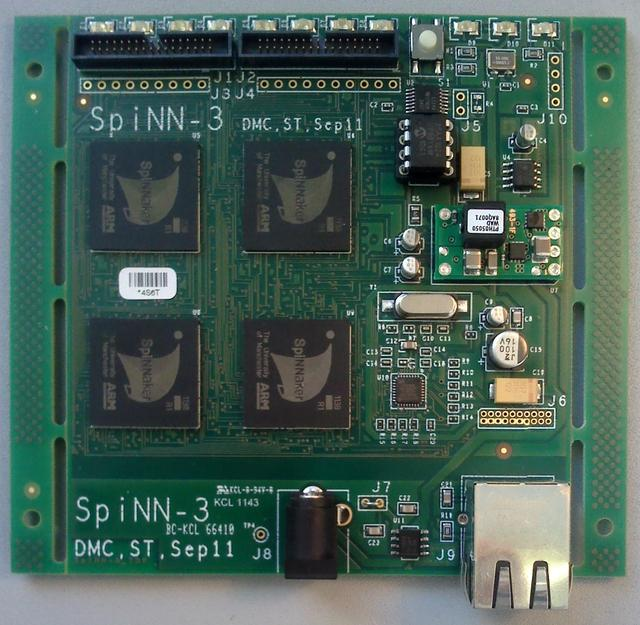
\includegraphics[width=\textwidth]{spin3}
            \end{figure}
        \end{columns}
    \end{frame}
    
%    \begin{frame}{Why SpiNNaker?} %{hello}
%        %More content goes here
%        \vspace*{-2em}
%        \begin{columns}[c] % the "c" option specifies center vertical alignment
%            \column{.666\textwidth} % column designated by a command
%            \begin{itemize}
%                \item Real-time simulation
%                \item Software models
%                \item Energy efficient
%            \end{itemize}
%            \column{.333\textwidth}
%            \begin{figure}
%                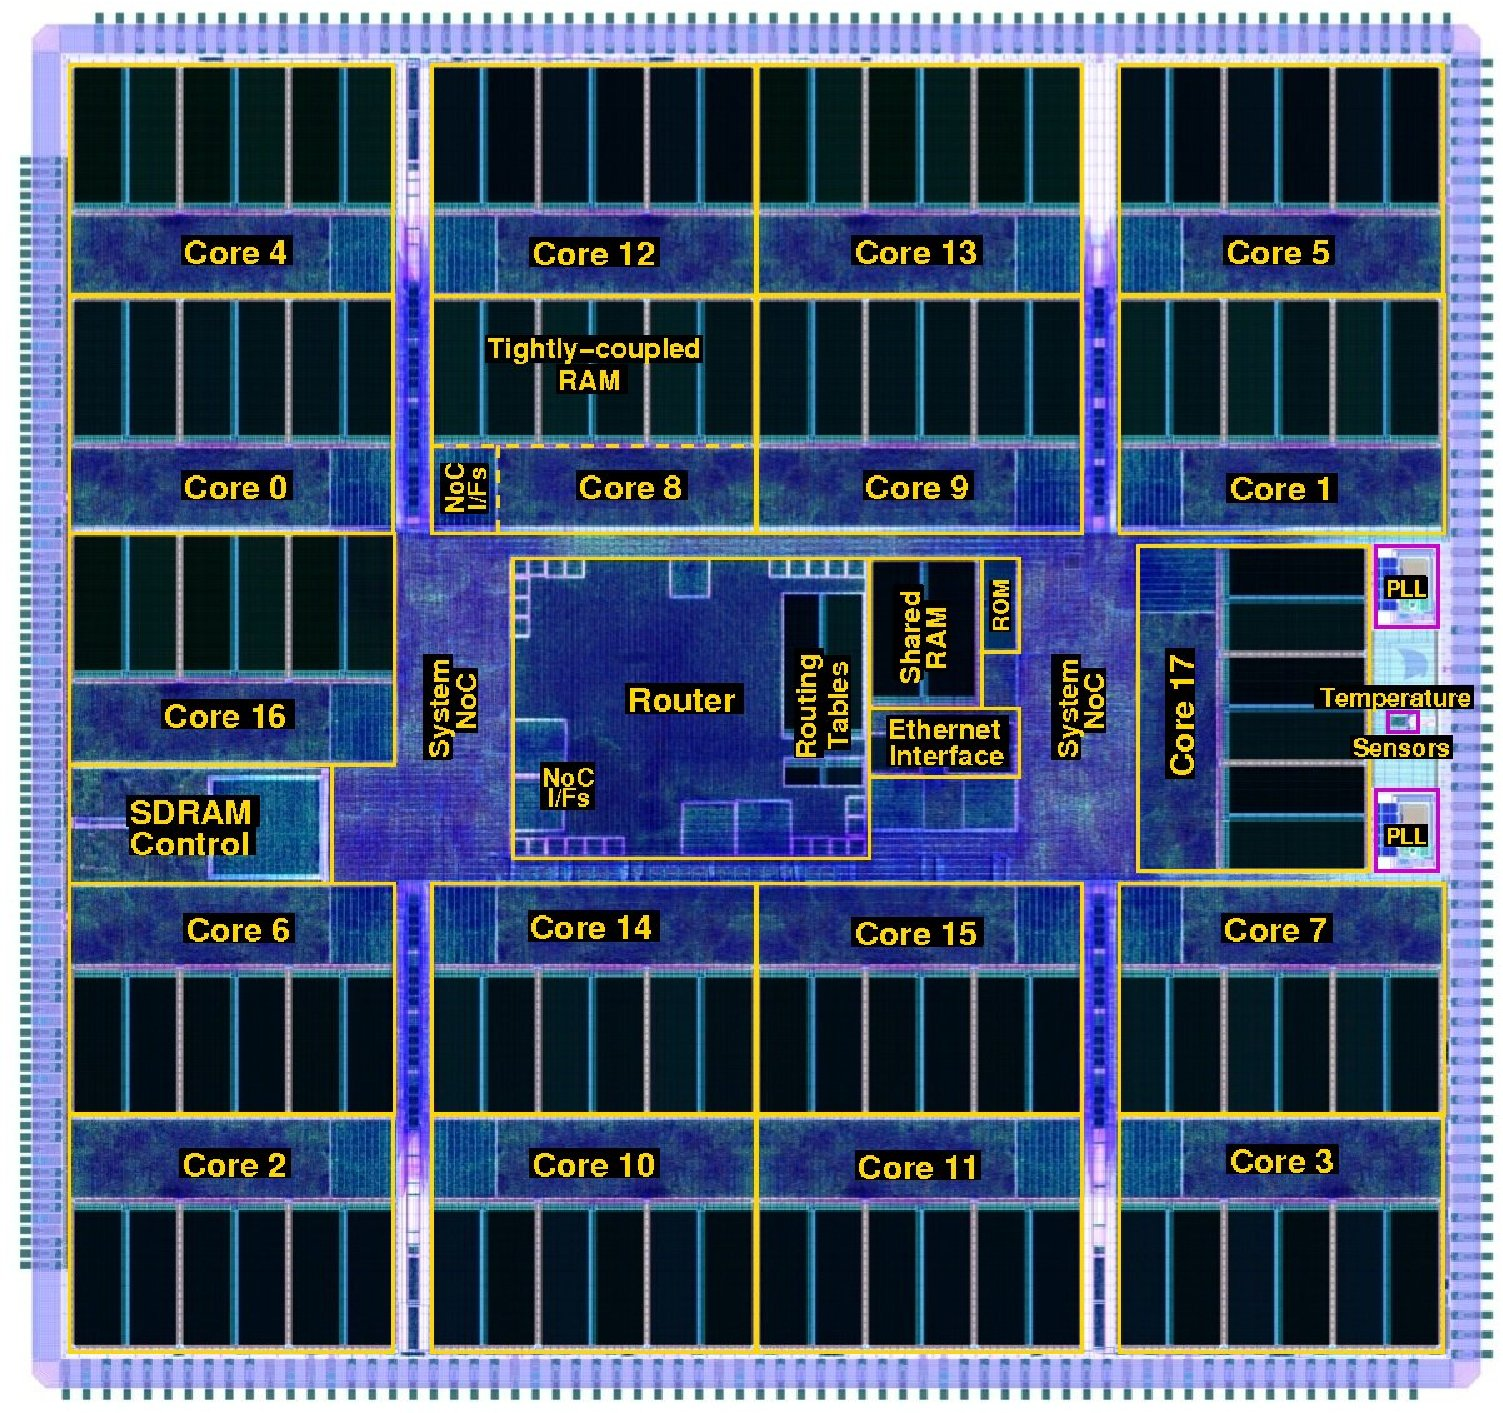
\includegraphics[width=\textwidth]{spinn_labeled}
%            \end{figure}
%        \end{columns}
%    \end{frame}
            
        
    \begin{frame}{Current work}
      %More content goes here
        \vspace*{-4em}
        \begin{figure}
            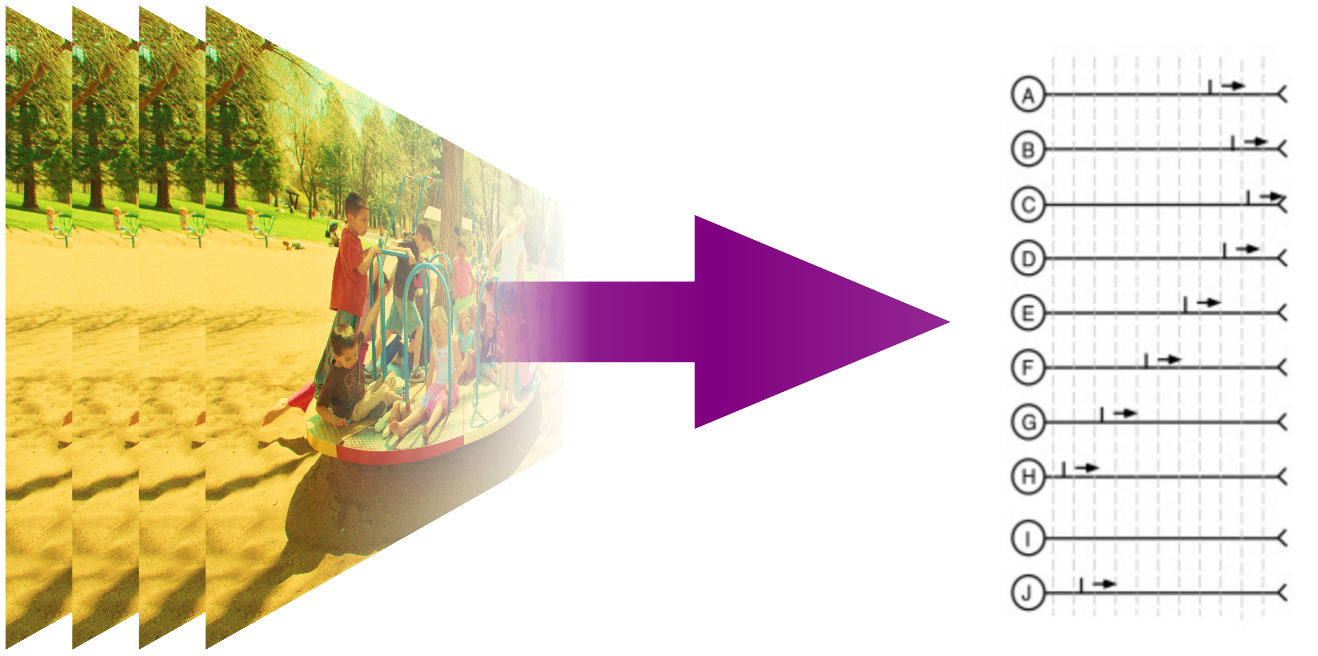
\includegraphics[scale=0.3]{./images-to-spikes}
        \end{figure}
        \vspace*{-0.4em}
        \hspace*{0.05\textwidth}
        \begin{minipage}{0.9\textwidth}
          \centering \small Convert images/video from a frame-based camera to spike trains
        \end{minipage}
    \end{frame}

    \begin{frame}{Retina}
        %More content goes here
        \vspace*{-4em}
    \begin{figure}
        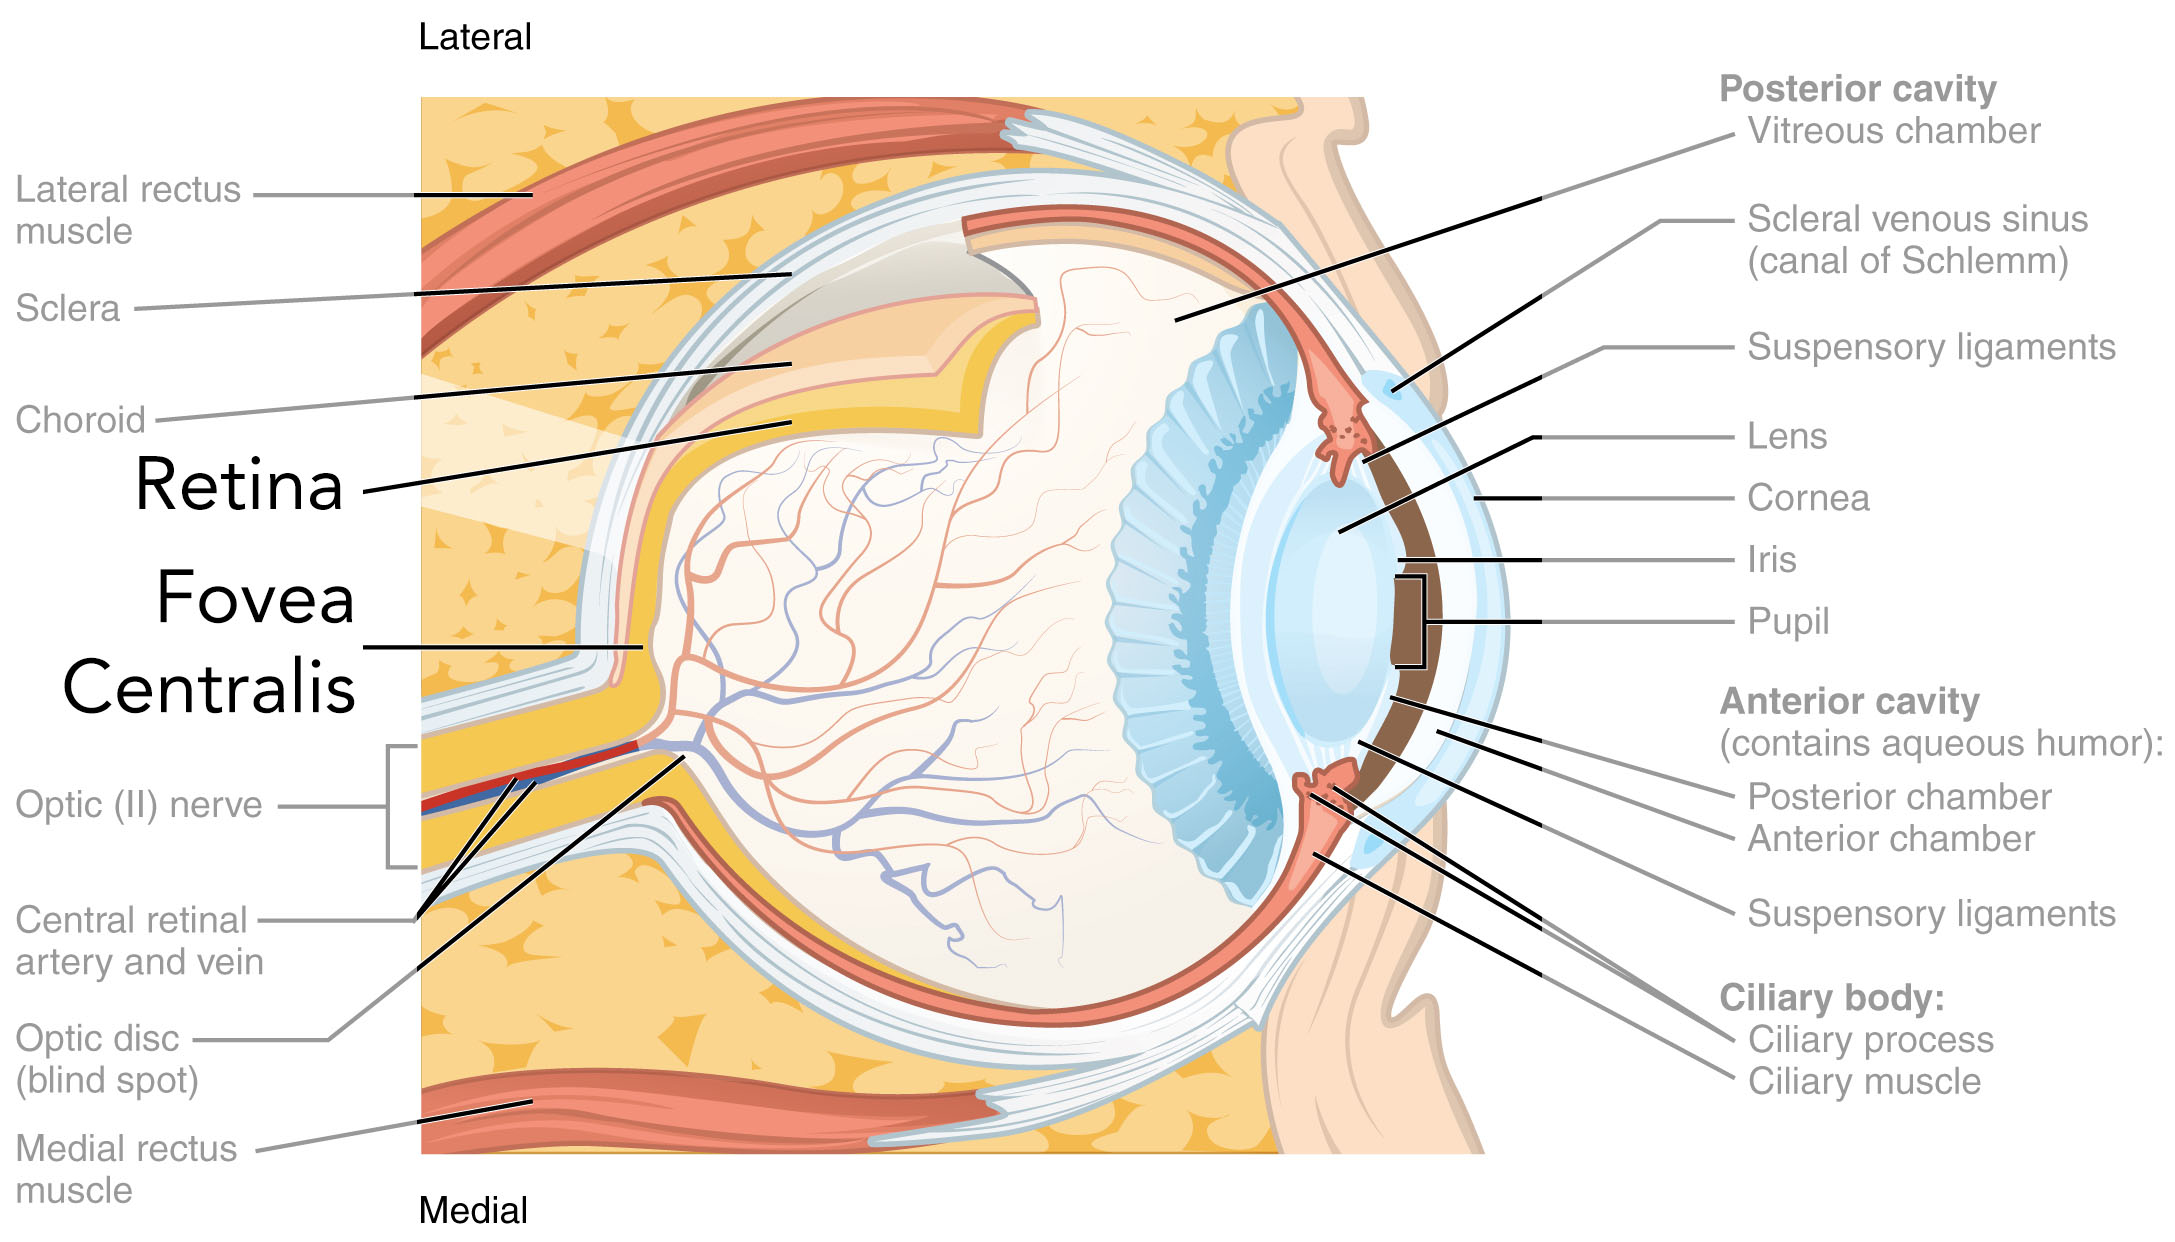
\includegraphics[width=1.1\textwidth]{eye-anatomy-detail}
        
    \end{figure}
    \end{frame}
    
    \begin{frame}{First retinal model}
        %More content goes here
        \vspace*{-3em}
        \begin{itemize}
            \item \textbf{Foveal pit} model with \emph{rank-ordered} output \footnote{\cite{basab}}
            \item Center-surround behaviour
        \end{itemize}
        \begin{figure}
          \vspace*{-1.em}
          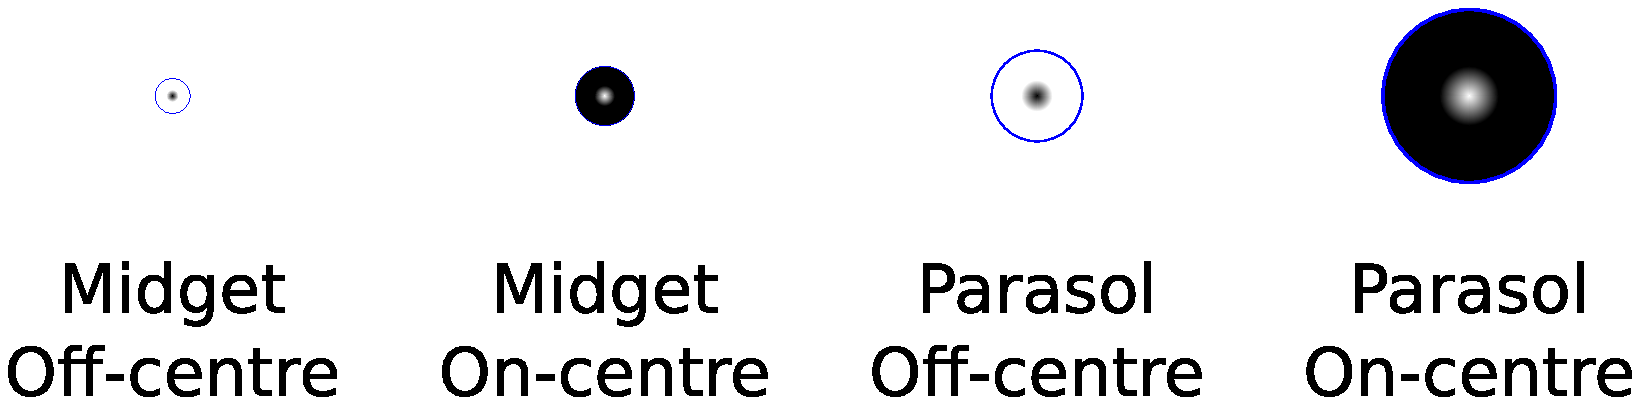
\includegraphics[scale=0.35]{./retina-model-table}
        \end{figure}
    \end{frame}
    
    \begin{frame}{Foveal pit connections}
      %More content goes here
      \vspace*{-4em}
      \begin{figure}
        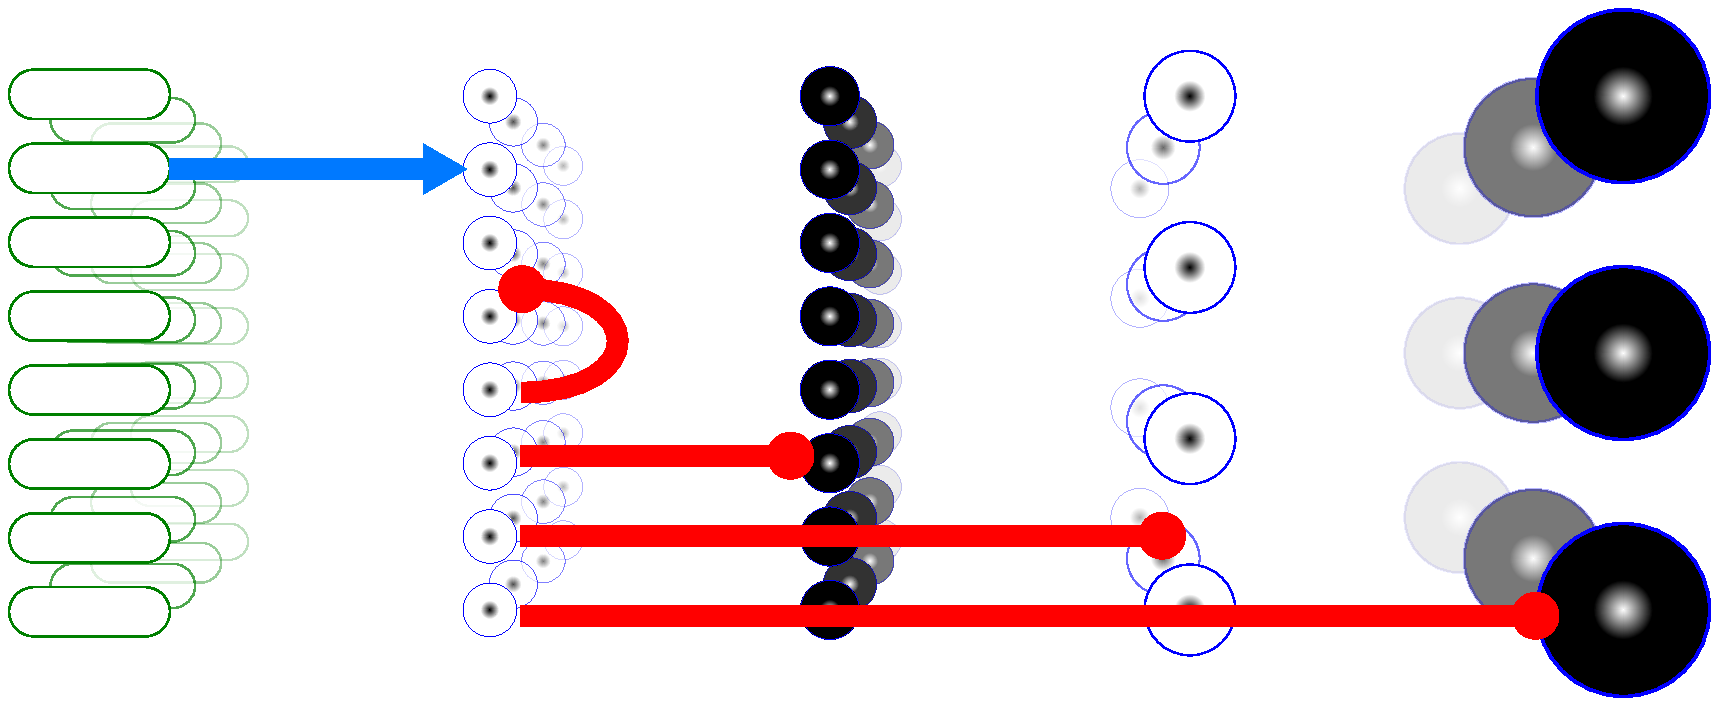
\includegraphics[scale=0.35]{./retina-model}
      \end{figure}
      \vspace*{-0.5em}
      %      \hspace*{0.05\textwidth}
      \begin{minipage}{\textwidth}
        \begin{itemize}
          \normalsize           
          \item Excitatory connections from photoreceptors to ganglion cells.
          \item Inhibitory connections to and from ganglion cells.
        \end{itemize}
      \end{minipage}
    \end{frame}

    \begin{frame}{FoCal}
      %More content goes here
      \vspace*{-3em}
      \begin{minipage}{0.48\textwidth}
        \centering
        \begin{figure}
          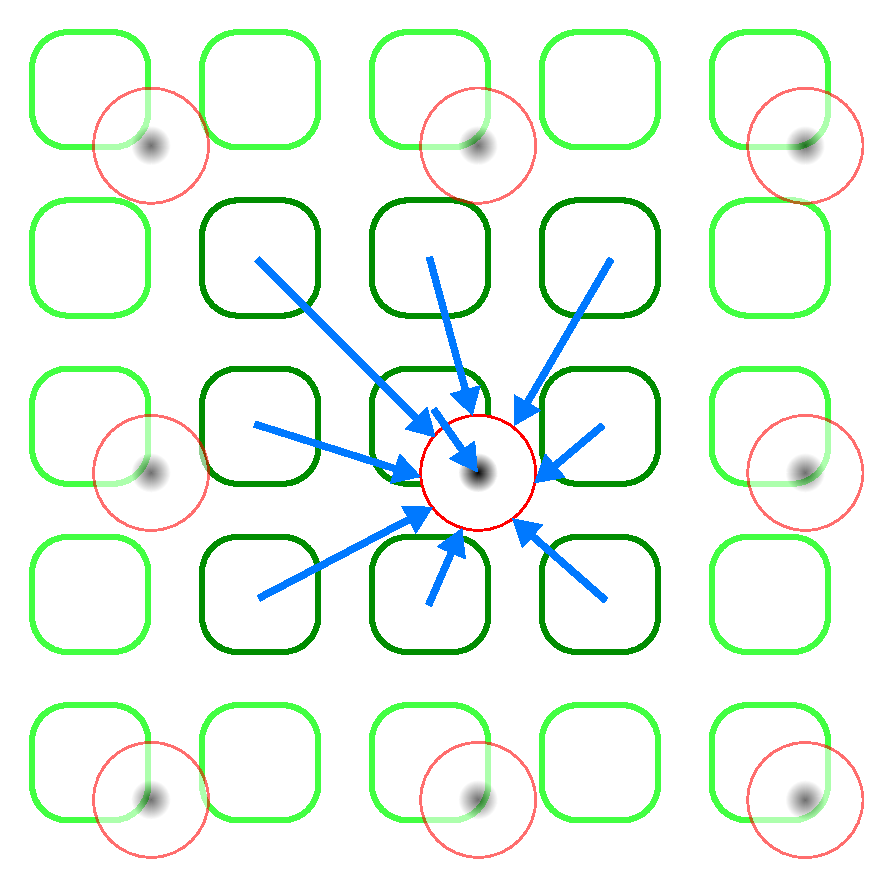
\includegraphics[scale=0.3]{./single_cell_midget-off}
        \end{figure}
        \vspace*{-1em}
        Excitatory\\
        Convolution\\
        Parallel
      \end{minipage}
      \begin{minipage}{0.48\textwidth}
        \centering
        \begin{figure}
          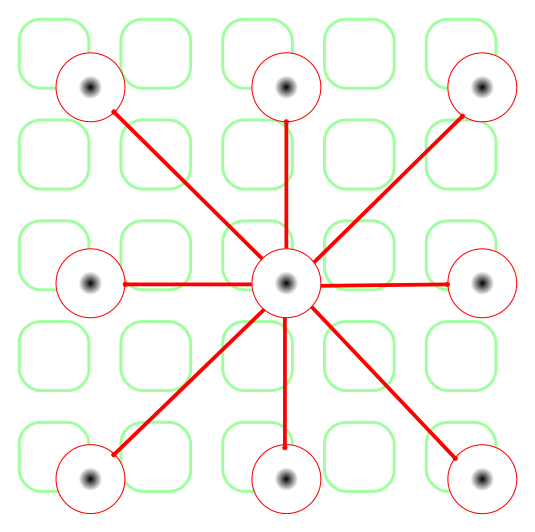
\includegraphics[scale=0.3]{./single_cell_midget-off-inh}
        \end{figure}
        \vspace*{-1em}
        Inhibitory\\
        Adjust weights\\
        Serial
      \end{minipage}
    \end{frame}

    \begin{frame}{FoCal - convolution}
      %More content goes here
      \vspace*{-3em}
      \centering
        \begin{figure}
          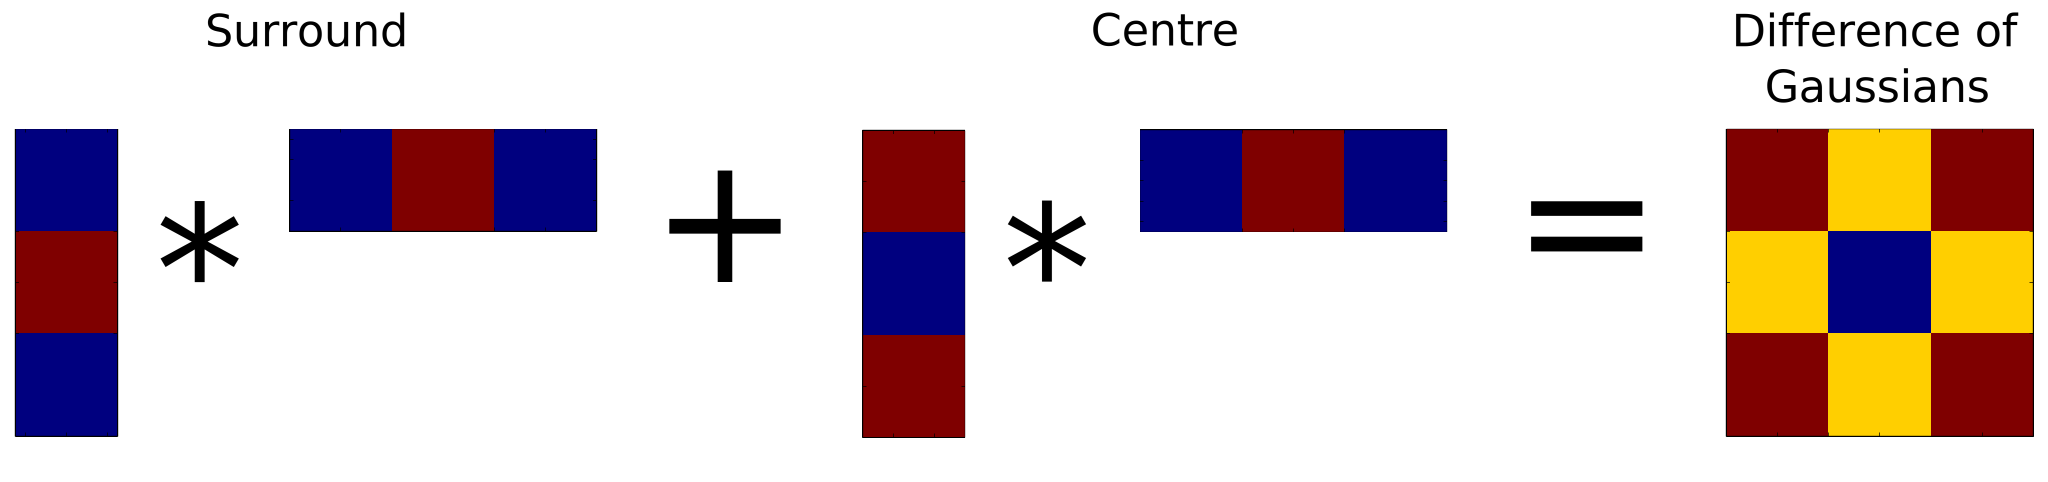
\includegraphics[width=\textwidth]{./separated}
        \end{figure}
        \vspace*{-1em}
        Separated, four 1D convolutions instead of one 2D. 
        Better for parasol cells. 
    \end{frame}
    
    \begin{frame}{FoCal - convolution}
      %More content goes here
      \vspace*{-5em}
      \centering
      \begin{figure}
        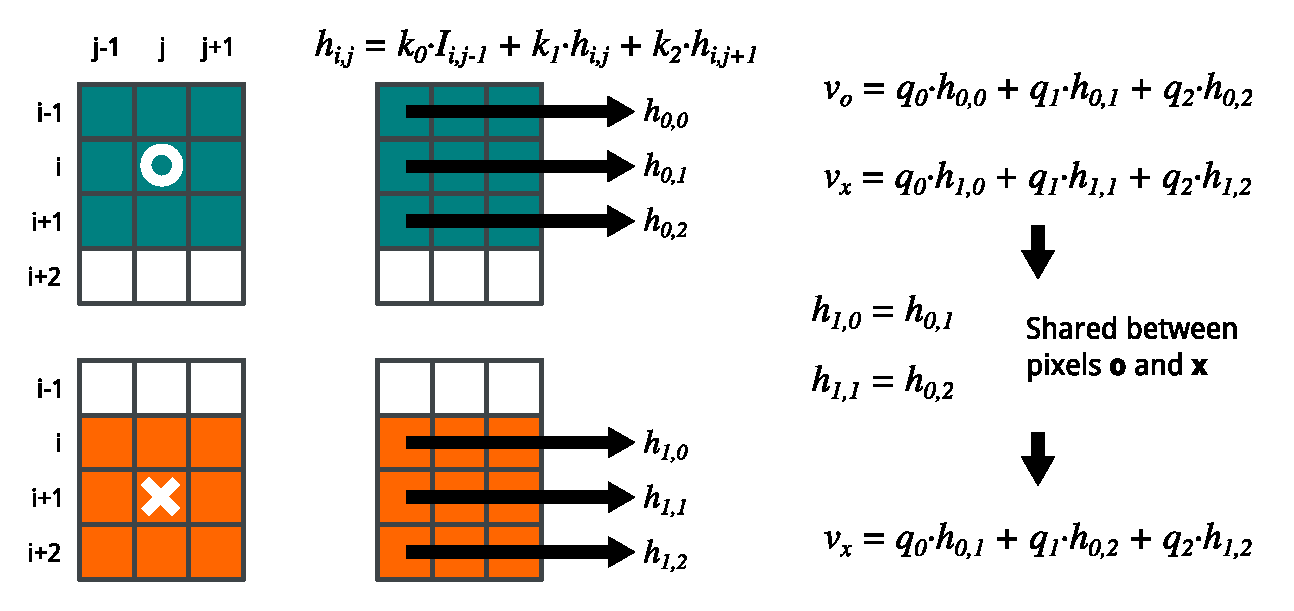
\includegraphics[width=\textwidth]{./tiled-conv}
      \end{figure}
      \vspace*{-1em}
        Tiled, separability based, reuse calculations. Better for midget cells.
      
    \end{frame}
%    \begin{frame}{Foveal pit (part 1)}
%      %More content goes here
%       \vspace*{-5em}
%       \begin{columns}[c] % the "c" option specifies center vertical alignment
%         \column{.67\textwidth}
%         \begin{itemize}
%           \item Excitatory connections
%           \item Convolution
%           \item In parallel
%          \end{itemize}
%         \column{.6\textwidth}
%          \begin{figure}
%            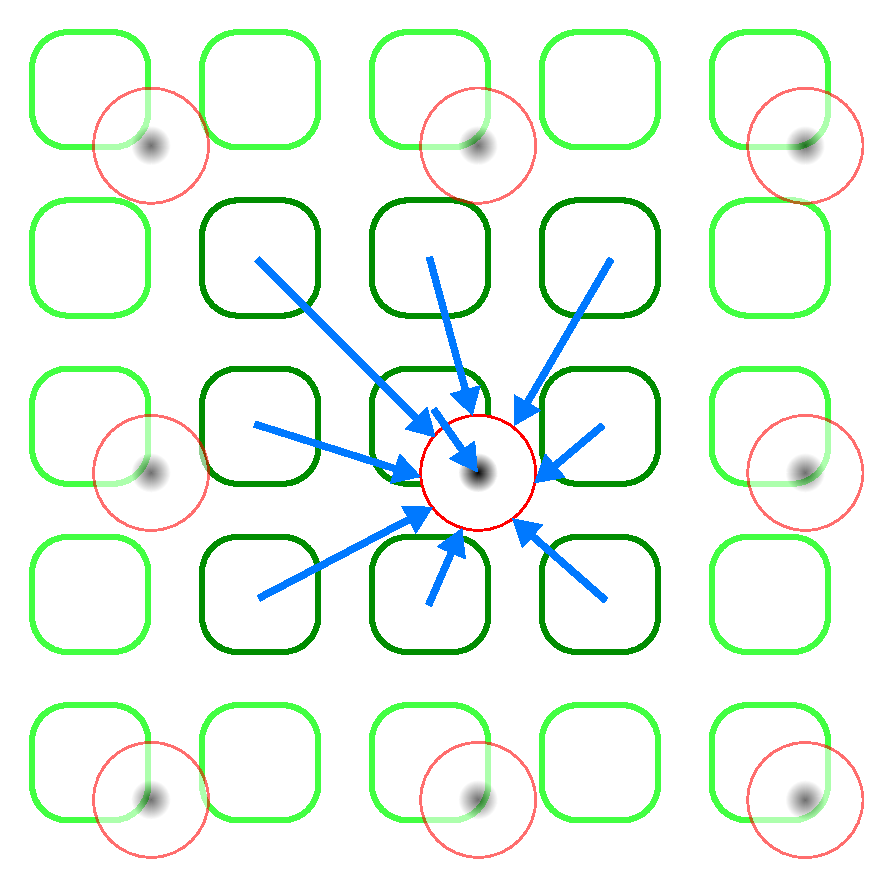
\includegraphics[scale=0.25]{./single_cell_midget-off}
%          \end{figure}
%      \end{columns}
%    \end{frame}
%    
%    \begin{frame}{Foveal pit (part 2)}
%      %More content goes here
%      \vspace*{-5em}
%      \begin{columns}[c] % the "c" option specifies center vertical alignment
%        \column{.67\textwidth}
%        \begin{itemize}
%          \item Inhibitory connections
%          \item Weight adjustment based on correlation
%          \item Serial
%        \end{itemize}
%        \column{.6\textwidth}
%        \begin{figure}
%          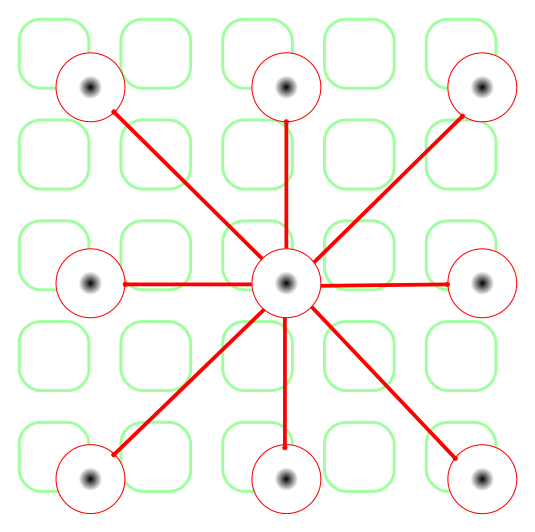
\includegraphics[scale=0.25]{./single_cell_midget-off-inh}
%        \end{figure}
%      \end{columns}
%    \end{frame}


    \begin{frame}{Foveal pit results}
      \vspace*{-4em}
      \begin{itemize}
        \item Convolution of 4 cell types using OpenCL @ 12 fps (\texttildelow60 MOps/sec )
        \item Issues: Memory transfers for huge kernels
      \end{itemize}
      \vspace*{-1em}
      \begin{figure}
        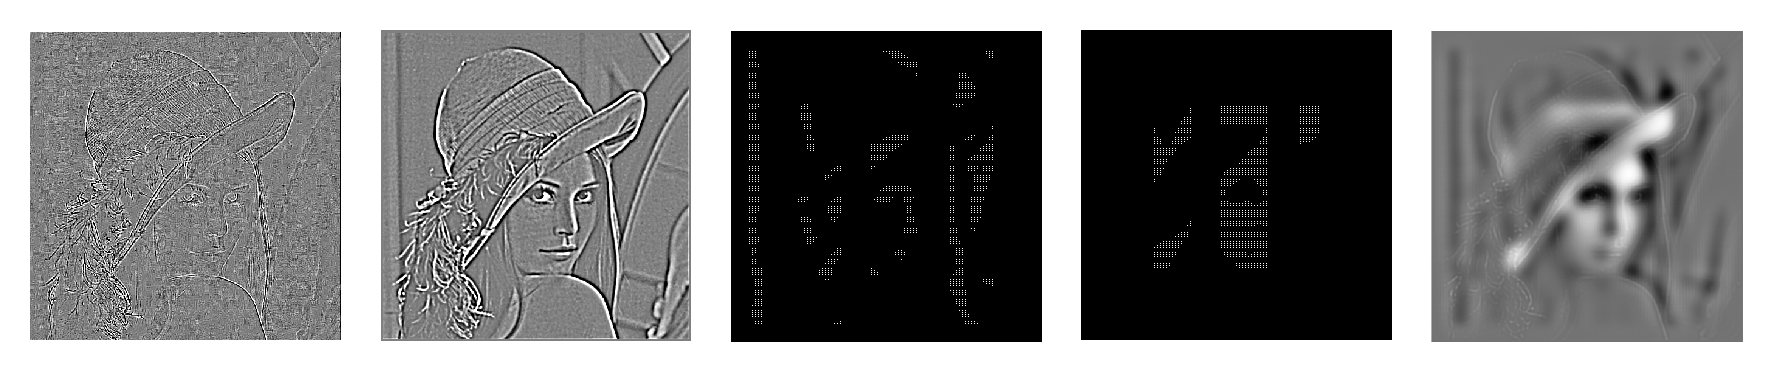
\includegraphics[width=\textwidth]{conv-imgs}
      \end{figure}
    \end{frame}
    \begin{frame}{Foveal pit results}
      \vspace*{-3em}
      \begin{itemize}
        \item Issues: massive connectivity (\texttildelow3.4 billion) or serial process
        \item Neural approach with SpiNNaker
      \end{itemize}
      \vspace*{-1em}
      \begin{figure}
        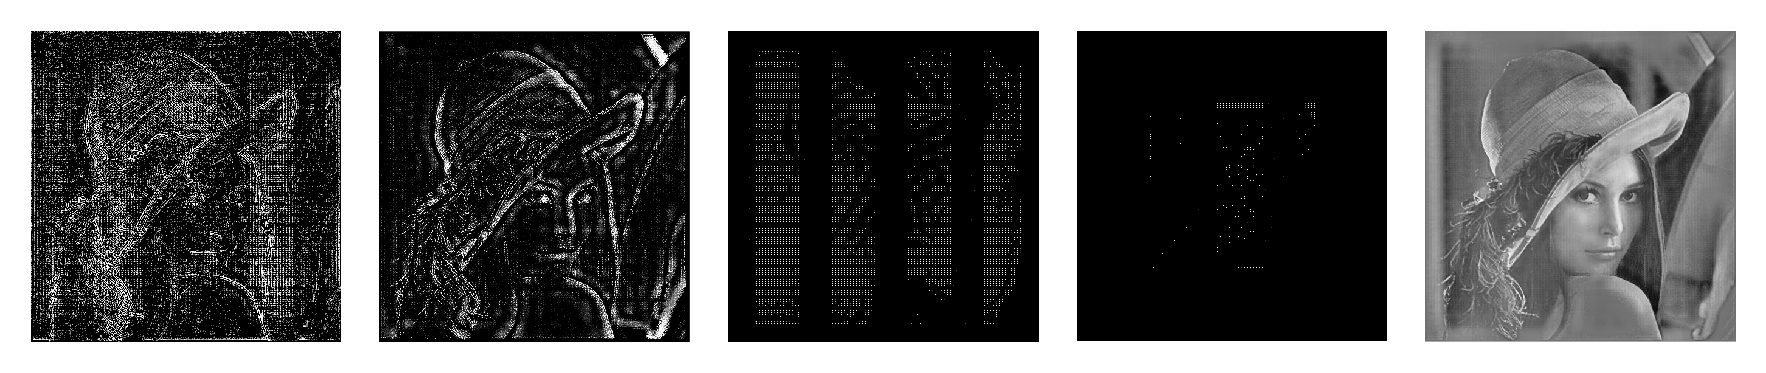
\includegraphics[width=\textwidth]{focal-imgs}
      \end{figure}
    \end{frame}

    \begin{frame}{Second retinal model}
      \vspace*{-2em}
      \begin{itemize}
        \item Emulate Dynamic Vision Sensor (DVS)
        \item Sense changes in illumination
        \item Per-pixel adaptive threshold
      \end{itemize}
      \vspace*{-1em}
      \begin{figure}
        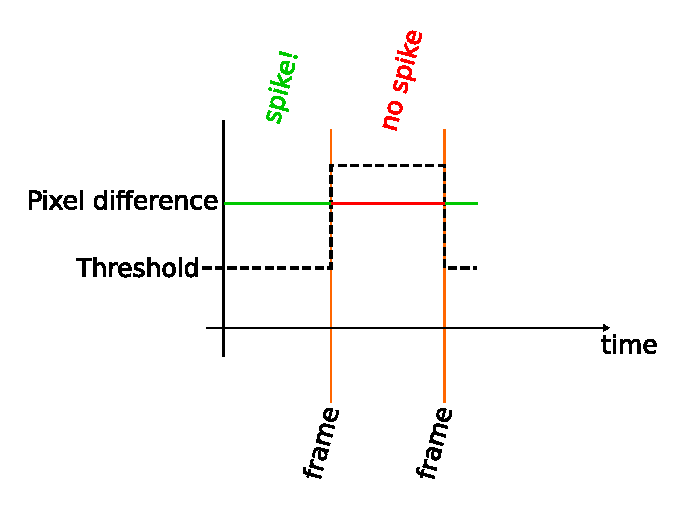
\includegraphics[width=0.6\textwidth]{DVSemu}
      \end{figure}
    \end{frame}

    \begin{frame}{DVS emulator}
      \vspace*{-2em}
      \hspace*{-2em}
      \begin{minipage}{0.66\textwidth}
        \begin{itemize}
          \item Camera bound dynamic range and spatial resolution
          \item Cheaper and easier to use!
        \end{itemize}
      \end{minipage}
      \begin{minipage}{0.33\textwidth}
        \vspace*{-1em}
        \begin{figure}
          \hspace*{0.1em}
          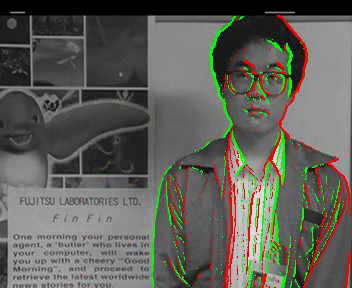
\includegraphics[scale=0.38]{dvs-emu-img}
        \end{figure}
      \end{minipage}
    \end{frame}

    \begin{frame}{Summary}
        %More content goes here
        \vspace*{-3em}
        \begin{itemize}
          \item Real-time convolution is possible
          \item Working on SpiNNaker based FoCal
          \item Submitted for paper and poster
          \item DVS emulator, working @ 25 fps on OpenCL ... but needs more testing
        \end{itemize}
    \end{frame}

    \begin{frame}{The Future}
      %More content goes here
      \vspace*{-3em}
      \begin{itemize}
        \item Keep improving video sources, custom hardware
        \item Polychronization
        \item Learning with time-based spikes
        \item Spatio-temporal patterns
      \end{itemize}
    \end{frame}

    \begin{frame}{Polychronization}
      %More content goes here
      \vspace*{-3em}
      \begin{itemize}
        \item Networks with delays
        \item Spike-timing encoding
        \item Connectivity similar to FoCal
      \end{itemize}
    \end{frame}


   \begin{frame}{The End}
      %More content goes here
    \begin{center}
        \vspace*{-3em}
        {\Large Thank You!}\\
        \vspace*{0.5em}
        Contact me:\\[1em]
%        chanokin@gmail.com\\
        {\Large \textbf{pinedagg@cs.man.ac.uk}}\\
    \end{center}
  \end{frame}
        
\end{document}
